% paper.tex - publication for Monthly Notices of the Royal Astronomical Society

\documentclass[useAMS,usenatbib]{mn2e}
\usepackage{txfonts}
\usepackage{graphicx}
\usepackage{natbib}

\def\del#1{{}}
%\def\del#1{{\bf (DELETED TEXT)}}
%\def\C#1{#1}
\def\C#1{{\bf #1}}

\sloppy

% --- macros --- %
\newcommand{\icm}{intra-cluster medium}
\newcommand{\cmb}{cosmic microwave background}

% --- journals --- %
\newcommand{\aap}{A{\&}A}
\newcommand{\aaps}{A{\&}AS}
\newcommand{\aj}{AJ}
\newcommand{\apj}{ApJ}
\newcommand{\apjl}{ApJL}
\newcommand{\apjs}{ApJS}
\newcommand{\apss}{Ap{\&}SS}
\newcommand{\araa}{ARA{\&}A}
\newcommand{\prd}{Phys. Rev. D}
\newcommand{\pre}{PRE}
\newcommand{\mnras}{MNRAS}
\newcommand{\ssr}{SSRv}
\newcommand{\nat}{Nature}
\newcommand{\physrep}{Phys.~Rep.}
\newcommand{\jcomp}{J.~Comput.~Phys.}

% --- christoph's commands --- %
\newcommand{\dd}{\mathrm{d}}
\newcommand{\bra}{\langle}
\newcommand{\ket}{\rangle}
\newcommand{\ltsima}{$\; \buildrel < \over \sim \;$}
\newcommand{\lsim}{\lower.5ex\hbox{\ltsima}}
\newcommand{\gtsima}{$\; \buildrel > \over \sim \;$}
\newcommand{\gsim}{\lower.5ex\hbox{\gtsima}}
\newcommand{\eps}{\varepsilon}

% --- Anders's commands --- %
\newcommand{\ev}{\mathrm{eV}}
\newcommand{\gev}{\mathrm{GeV}}
\newcommand{\mev}{\mathrm{MeV}}
\newcommand{\tev}{\mathrm{TeV}}
\newcommand{\mpc}{m_{\mathrm{p}}c}
\newcommand{\mpcc}{m_{\mathrm{p}}c^2}
\newcommand{\p}{\mathrm{p}}
\newcommand{\Pp}{\mathrm{P}_\mathrm{p}}
\newcommand{\Pe}{\mathrm{P}_\mathrm{e}}
\newcommand{\pp}{p_\mathrm{p}}
\newcommand{\pe}{p_\mathrm{e}}
\newcommand{\br}{\bold{r}}
\newcommand{\e}{\mathrm{e}}
\newcommand{\ii}{\mathrm{i}}
\newcommand{\inj}{\mathrm{inj}}
\newcommand{\pd}{\partial}
\newcommand{\CR}{\mathrm{CR}}
\newcommand{\gas}{\mathrm{gas}}
\newcommand{\mr}{\mathrm}
\newcommand{\DM}{\mathrm{DM}}
\newcommand{\ISM}{\mathrm{ISM}}
\newcommand{\ICM}{\mathrm{ICM}}
\newcommand{\CMB}{\mathrm{CMB}}
\newcommand{\IC}{\mathrm{IC}}
\newcommand{\mecc}{m_\e c^2}
\newcommand{\mug}{\mathrm{\mu G}}
\newcommand{\rvir}{R_{200}}
\newcommand{\B}{\mathrm{B}}
\newcommand{\ma}{\mathrm{max}}
\newcommand{\low}{\mathrm{low}}
\newcommand{\gae}{\gamma_\mathrm{e}}
\newcommand{\gap}{\gamma_\mathrm{p}}
\newcommand{\gam}{\gamma}
\newcommand{\tend}{t_f}
\newcommand{\mach}{\mathcal{M}}



% --- title --- %
\title{The origin of cosmic-ray electrons in cluster outskirts}

\author[A. Pinzke, S.P. Oh and C. Pfrommer] 
  {Anders Pinzke$^1$\thanks{e-mail:apinzke@physics.ucsb.edu (AP); peng@physics.ucsb.edu (PO);pfrommer@h-its.org (CP)}, S. Peng Oh$^1$\footnotemark[1],
    and Christoph Pfrommer$^2$\footnotemark[1]\\
    $^1$University of California - Santa Barbara,
  Department of Physics, CA 93106-9530, USA\\
    $^2$Heidelberg Institute for Theoretical Studies
  (HITS), Schloss-Wolfsbrunnenweg 33, DE - 69118 Heidelberg, Germany}
    

% --- document --- %
\begin{document}
\pagerange{\pageref{firstpage}--\pageref{lastpage}} \pubyear{2011}
\maketitle
\label{firstpage}


% --- abstract --- %
\begin{abstract}
  bla bla bla
\end{abstract}


% --- keywords --- %
\begin{keywords}
  magnetic fields, cosmic rays, radiation mechanisms: non-thermal, elementary
  particles, galaxies: cluster: general
\end{keywords}

% --- section: introduction --- %
\section{Introduction}
Diffuse radio emission in clusters falls into two broad classes: smooth, centrally located and unpolarized radio halos \citep[][ and references therein]{ferrari08}, and elongated, significantly polarized and steep spectrum radio relics� which are seen at cluster outskirts \citep[][ and references therein]{kempner04}. Both are associated with merging clusters. Radio relics are thought to come in distinct classes: fossil AGN radio lobes, which may have been re-energized by compression (‘radio phoenix’; \citet{ensslin01}), and those produced by direct Fermi-I particle acceleration at accretion/merger shocks (radio gischt; \citet{ensslin98,miniati01}). Many radio relics have now been seen ($\sim 45$; for a recent compilation, see \citet{nuza11}); the number could increase dramatically with upcoming low frequency radio surveys proposed for the Low Frequency Array (LOFAR), the Westerbork Synthesis Radio Telescope (WSRT), and farther in the future, Square Kilometer Array (SKA). Using numerical simulations combined with an semi-analytic model for radio emission calibrated to existing number counts, \citet{nuza11} estimate that LOFAR and WSRT could discover $\sim 2500$ relics and $\sim 900$ relics respectively. The time is therefore ripe to understand how we can best mine these future surveys.   

In this paper, we focus on radio gischt, which trace structure formation shock waves. They therefore can illuminate the nature of cosmic accretion/mergers, as well as shock amplification of large-scale  magnetic fields \citep{pfrommer08, hoeft08, battaglia09, skillman11}. Perhaps even more importantly, they allow us to probe in detail the efficiency of shock acceleration in a diffuse, low Mach number ($\mach \sim 2-4$) regime far different from the high Mach number regimes probed in our Galaxy and supernova remnants. Whilst this remains poorly understood, observations seem to suggest an electron acceleration efficiency significantly in excess of naive theoretical expectiations. In this paper, we explore a promising explanation: the existence of a seed population of low energy ($\gamma \sim 200$) relic relativistic electrons from high redshift which are reaccelerated by low-redshift shocks.  

A recent spectacular example of radio gischt is CIZA J2242.8+5301, the 'sausage relic'  \citep{van-weeren10}, a large ($\sim 2$ Mpc long; located $\sim 1.5$ Mpc from the cluster center) double radio relic system. The post-shock radio spectral index was used to infer the particle spectral slope and hence the shock compression ratio and Mach number ($\mach \sim 4.6$), while the decrease in the spectral index (from $\sim 0.6$ to $\sim 2.0$ across the relic� narrow $\sim 55$ kpc width) toward the cluster center---spectral aging due to synchrotron and inverse Compton losses---was used to infer magnetic field strengths of $\sim 5 \, \mu$G. The strong ($\sim 50-60 \%$) polarization can be attributed to magnetic field frozen into the compressed ICM, which has been aligned parallel to the shock. The properties of this and similar systems are distinct from fossil radio plasma, which are smaller, have curved, steeper spectra (due to aging), and lobe-like morphology. The power-law spectral index, spectral gradient, and enormous extent clearly support a diffusive shock acceleration (DSA) origin. 

However, this then presents a puzzle. Cosmological simulations show that while gas initially undergoes strong shocks (up to $\mach \sim 10^{3}$) accreting onto non-linear structures and filaments, shocks in the ICM and cluster outskirts are relatively modest ($\mach \sim 1-5$), since the gas has already reached sub-keV temperatures \citep{ryu03,pfrommer06,skillman08}. While DSA is efficient in accelerating particles in the thermal Maxwellian tail at high Mach numbers \citep{bell78,drury83}, and as confirmed in observations of supernova remnants \citep{parizot06,reynolds08}, at lower Mach numbers the efficiency of DSA is known to plummet exponentially {\bf SPO: should we include a figure of this? To me this paper is motivated by 2 figures, that of the acceleration efficiency as a function of Mach number and the cooling time as a function of energy---we could put it in 1 figure.} Indeed, in the test-particle regime where suprathermal particles undergo acceleration via a thermal leakage process (which compare well against kinetic DSA simulations) the acceleration efficiency for weak shocks $\mach \sim 3$ is extremely small; the fraction of protons accelerated is $\sim 10^{-4}-10^{-3}$, and cosmic ray proton pressure is $\lsim 1\%$ of the shock ram pressure \citep{kang11}. The acceleration efficiency of electrons at low Mach numbers is likely to be far smaller still. The injection problem for thermal electrons already known to be severe at high Mach numbers, due to the smaller gyroradius of thermal electrons: the relative acceleration efficiency of cosmic ray electrons is lower by $\sim 10^{-2}$ as in the Galaxy \citep{schlickeiser02} or even $\sim 10^{-4}$ as in supernova remnants \citep{morlino09}). These relative efficiencies likely plummets further at low Mach numbers. These considerations appear to contradict the appearance of bright radio relics, and perhaps suggest that our understanding of DSA at low Mach numbers is incomplete (for recent progress, see \citep{gargate12}). 

A possible solution is if there is a pre-existing population of cosmic ray electrons with gyroradii comparable or larger than that of the shock thickness. In this case, injection from the thermal pool is no longer an issue \citep{markevitch05,giacintucci08,kang11}; here,  \citet{kang11} show that re-acceleration should dominate over fresh injection. %\footnote{Turbulent re-acceleration, which is thought to operate at lower Mach numbers, also requires a seed population of relativistic particles}. 
DSA has a much larger effect on radio emission than adiabatic compression; including the downstream magnetic field amplification, synchrotron emission could be boosted by a factor $\sim 100-1000$ for $\mach \sim 3$ \citep{kang11}. Thus, the luminosity function of radio gischt will be strongly modified by the presence or absence of a seed relativistic electron population, whose existence has never been directly demonstrated. In this paper, we use our existing high-resolution SPH simulations of cosmic-ray protons in clusters \citep{pinzke10} to infer whether structure formation shocks could generate them\footnote{They could also have a non-gravitational origin, such as AGN injection, though the filling factor at these large radii is likely to be small.}, taking into account the effects of electron cooling. Note that DSA operates identically on relativistic particles of the same rigidity ($R=pc/Ze$), so the injected proton and electron spectrum are the same, modulo their relative acceleration efficiency, which we conservatively calibrate off Galactic observations.%\footnote{Note, however, that at energies where protons are subrelativistic, the electron spectrum has to be obtained from the proton spectrum by extrapolating the latter from the relativistic regime.} 
In the low-density outskirts of clusters, proton loss timescales are several Hubble times, so we can directly derive the injected energy to each SPH CRp particle directly from our existing simulation snapshots and derive an appropriate scaled injection of CR electrons (CRe). Unlike CRp, Coulomb and inverse Compton/synchrotron loss processes are more efficient and have to be taken into account (IC off the CMB, which has an equivalent energy density of $B=3.24 (1+z)^{2} \mu$G, should dominate in the outer regions). We evolve the time-dependent cosmic-ray energy equation to track the evolving distribution function of CRe. In Fig \ref{fig:ensslin}, we can see that the $\sim 10$ GeV CRe  responsible for $\sim$GHz emission in a $\mu$G field has energy loss timescales of $\sim 10^{8}$yr, but a large population of $\sim 100$ MeV electrons could build up. Note that secondary CRe which arise from hadronic interactions of CRp are not thought to be significant at these low densities, though for a dissenting view, see \citet{keshet10}. We calculate the abundance of such seed electrons from structure formation shocks in the cluster outskirts. In general, we find that they are, reaffirming radio gischt as a reliable tracer of large scale shocks and magnetic fields


\begin{figure}[ht]
\begin{center}
%\resizebox{!}{5.5cm}{\includegraphics{./figures/ensslin.eps}}
%%\resizebox{!}{5.5cm}{\includegraphics{ensslin2.pdf}}
%\resizebox{!}{5.0cm}{\includegraphics{circles.pdf}}
%%\hspace{0.05cm}
%%%\vspace{-1cm} 
\end{center}
\caption{Cooling time of CR electrons (left panel) and CR protons (right panel) for typical conditions in the ICM. CRe can only survive for a Hubble time in the underdense outskirts of clusters; $\sim 100$MeV electrons should be the most long-lived. By contrast, CRp above 10 GeV can survive on cosmological timescales. From \citet{ensslin11}. {\bf I stole this figure from Ensslin�should we make our own?}}
\label{fig:ensslin} % caption for the whole figure
\end{figure}


The outline of this paper is as follows. {\bf Blah blah, fill in once paper is complete}. 

\section{Order of Magnitude Estimates: The Production and Survival of Relic Electrons} 
\label{sect:estimates}


\section{Simulations}
\label{sect:simulations}
Our simulations were performed in a $\Lambda$CDM universe using the
cosmological parameters: $\Omega_{\mr m}=\Omega_\DM + \Omega_{\mr
  b}=0.3, \, \Omega_{\mr b}=0.039, \, \Omega_\Lambda=0.7, \, h=0.7, \,
n_{\mr s}=1$, and $\sigma_8=0.9$. The total matter density in units of
the critical density of the universe $\rho_{\rm crit}$ is denoted by
$\Omega_{\mr m}$, the baryonic density by $\Omega_{\mr b}$, the DM
density by $\Omega_\DM$ and the cosmological constant today is denoted
by $\Omega_\Lambda$. The critical density, $\rho_{\rm crit}=3H_0/(8\pi
G)$, where the present day Hubble constant $H_0=100\, h \, \mr{km}\,
\mr{s}^{-1} \, \mr{Myr}^{-1}$. $n_{\mr s}$ represents the spectral
index of the primordial power-spectrum, and $\sigma_8$ denotes the
$rms$ linear mass fluctuation within a sphere of radius $8 \,h^{-1}
\mr{Mpc}$ extrapolated to $z = 0$. The simulations were carried out
with an updated and extended version of the distributed-memory
parallel TreeSPH code GADGET-2 \citep{2005MNRAS.364.1105S,
  2001NewA....6...79S}. Gravitational forces were computed using a
combination of particle-mesh and tree algorithms.  Hydrodynamic forces
are computed with a variant of the smoothed particle hydrodynamics
(SPH) algorithm that conserves energy and entropy where appropriate,
i.e. outside of shocked regions \citep{2002MNRAS.333..649S}.  Our
simulations follow the radiative cooling of the gas, star formation,
supernova feedback, and a photo-ionizing background \citep[details can
  be found in][]{2007MNRAS.378..385P}. We model the cosmic ray (CR)
physics in a self-consistent way \citep{pfrommer06,
  2007A&A...473...41E, 2008A&A...481...33J} and attach a CR proton
distribution function to each SPH fluid element. We include the
adiabatic CR transport process such as compression and rarefaction,
and a number of physical source and sink terms which modify the cosmic
ray pressure of each CR population separately. The most important
sources considered for injection are, diffusive shock acceleration at
cosmological structure formation shocks and shock waves in supernova
remnants, while the primary sinks are thermalization by Coulomb
interactions, and catastrophic losses by hadronization. For
simplicity, in this paper we do not take into account CRs injected
into the inter-stellar medium from supernova remnants (see Pinzke, Oh,
and Pfrommer, in prep. for a discussion of this topic).


\begin{table}
\caption{Cluster sample.}
\begin{tabular}{l l l l r r r}
\hline
\hline
Cluster & sim.'s & state$^{(1)}$ & $M_{\rm vir}^{(2)}$ & $\rvir^{(2)}$ & $kT_{\rm vir}^{(3)}$ & $\Delta t$$^{(4)}$\\
& & & [$\rmn{M}_\odot$] & [Mpc] & [keV] & \\
\hline
1  & g8a  & CC    & $2.6\times 10^{15}$ &   2.9~~ & 13.1 & 1.127 \\
2  & g1a  & CC    & $1.9\times 10^{15}$ &   2.5~~ & 10.6 & 1.127 \\
3  & g72a & PostM & $1.6\times 10^{15}$ &   2.4~~ & 9.4  & 100 Myr \\
4  & g51  & CC    & $1.5\times 10^{15}$ &   2.4~~ & 9.4  & 1.127 \\
                                                     
5  & g1b  & M     & $5.2\times 10^{14}$ &   1.7~~ & 4.7  & 1.127 \\
6  & g72b & M     & $2.2\times 10^{14}$ &   1.2~~ & 2.4  & 100 Myr \\
7  & g1c  & M     & $2.0\times 10^{14}$ &   1.2~~ & 2.3  & 1.127 \\
8  & g8b  & M     & $1.5\times 10^{14}$ &   1.1~~ & 1.9  & 1.127 \\
9  & g1d  & M     & $1.3\times 10^{14}$ &   1.0~~ & 1.7  & 1.127 \\
                                                     
10 & g676 & CC    & $1.3\times 10^{14}$ &   1.0~~ & 1.7  & 1.049 \\
11 & g914 & CC    & $1.2\times 10^{14}$ &   1.0~~ & 1.6  & 1.049 \\
12 & g1e  & M     & $9.1\times 10^{13}$ &  0.93   & 1.3  & 1.127 \\
13 & g8c  & M     & $8.5\times 10^{13}$ &  0.91   & 1.3  & 1.127 \\
14 & g8d  & PreM  & $7.8\times 10^{13}$ &  0.88   & 1.2  & 1.127 \\
\hline
\end{tabular}  \begin{quote}
 Notes:\\ (1) The dynamical state has been classified through a combined
 criterion invoking a merger tree study and the visual inspection of the X-ray
 brightness maps. The labels for the clusters are M--merger, PostM--post
 merger (slightly elongated X-ray contours, weak cool core (CC) region developing),
 PreM--pre-merger (sub-cluster already within the virial radius), CC--cool
 core cluster with extended cooling region (smooth X-ray profile).  (2) The
 virial mass and radius are related by $M_\Delta(z) = \frac{4}{3} \pi\,
 \Delta\, \rho_\rmn{crit}(z) R_\Delta^3 $, where $\Delta=200$ denotes a
 multiple of the critical overdensity $\rho_\rmn{crit}(z) = 3 H (z)^2/ (8\pi
 G)$.  (3) The virial temperature is defined by $kT_{\rm vir} = G M_{\rm vir} \,
 \mu\, m_\p / (2 R_{\rm vir})$, where $\mu$ denotes the mean molecular weight.
 (4) Time difference between output snapshots; in units of Myr for g72, and 
 remaining clusters show the ratio of the cosmological scale factor between 
 two snapshots.
\end{quote}
\label{tab:cluster_sample}
\end{table}


\section{Method}
\label{sect:method}
In this section we explain both the method that we use to derive the
CR electron distribution function that builds up during the structure
formation process of galaxy clusters, and the formalism for
calculating synchrotron emission from in galaxy cluster that is
undergoing a merger at low redshifts.

Our scheme is summarized in descending order by the following bullet points:
\begin{itemize}
\item derive CR proton distribution function from each simulation output at different time $t$
\item calculate injected CR proton population between snapshots 
\item convert injected protons to injected electrons
\item evolve each injected CR electron population to a later time $\tend$ by
  accounting for losses (Coulomb, inverse Compton, and adiabatic)
\item add up the CR electron distribution for all SPH particles at time $\tend$
\item re-accelerate CR electron distribution function at time $\tend$
  using typical values for a merging shock in cluster outskirts
\item calculate the synchrotron radio emission from radio relic
\end{itemize}

\subsection{CR protons}
The CR protons in the simulations are represented by a one-dimensional
isotropic distribution function \footnote{The three dimensional
  distribution function is given by $4\pi \int f(\gam)\, \gam^2\, \dd \gam$.}
given by
\begin{equation}
  \label{eq:f_p}
  f_\p(\gap) = \frac{\dd^2 N_\p}{\dd \gap\,\dd V} = 
  C\, \gap^{-\alpha}\,\theta(\gap-q)\,, 
\end{equation}
and the Lorentz factor $\gap \approx P_\p/m_\p c$, where we have
normalized the proton momentum $P_\p$ with the proton mass
$m_\p$. Here $q$ is the mass normalized momentum cutoff, $\alpha$ the
spectral index, and $C$ the normalization of the distribution function
in units of density.

To improve the numerical efficiency of the simulations the CR proton
distribution function is parameterized in terms of adiabatic invariant
momentum cutoff $q_0$ and the adiabatic invariant Lagrangian amplitude
of the spectrum $\tilde{C}_0$. We convert the adiabatic invariant
quantities to physical quantities through
\begin{equation}
  \label{eq:q0}
  q=\left(\frac{\rho}{\rho_0}\right)^{\frac{1}{3}}q_0\,,
\end{equation}
and
\begin{equation}
  \label{eq:C0}
  \tilde{C}=\left(\frac{\rho}{\rho_0}\right)^{-\frac{\alpha-1}{3}}\tilde{C}_0\,,
\end{equation}
where the convenient unitless redefinition of the CR proton amplitude
is given by
\begin{equation}
  \label{eq:Ct}
  \tilde{C}=C\,m_\p/\rho\,.
\end{equation}

\del{We select particles in the outskirts of clusters where the gas
  densities are low and hence the Coulomb cooling of the CR protons
  small.}

The CR electron distribution function can not be derived directly from
the CR protons because of the different timescales of loss
processes. Instead we first need to derive the injected CR proton
distribution function between each snapshot.  The injected
distribution function is calculated as the change in CR normalization
between a snapshot at time $t$ and an earlier time $t-\Delta t$:
\begin{eqnarray}
  \label{eq:finj}
f_\rmn{inj,p}(t,\gap) &=& \Delta C_0(t)\,\frac{\rho}{m_\p}\,
\gap^{-\alpha}\,,\qquad\rmn{where}\\
  \Delta  C_-(t) &=& C_0(t) - C_0(t-\Delta t)\,.
\end{eqnarray}
The time between snapshots is denoted by $\Delta t$ and is shown in
Table~\ref{tab:cluster_sample} for each simulated cluster. Note that
for most clusters we can not resolve the cooling timescale of CR
electrons, and hence we over estimate the abundance of electrons for
low and high momenta for some clusters (see
Figure~\ref{fig:e_spec_tests} for more details). Although, in the
region between $\gamma \sim (10-10^3)$ is small enough to resolve the
cooling processes.


\subsection{CR electrons}
The main difference between the CR electrons and CR protons comes from
the less efficient acceleration of the electrons due to the smaller
gyroradius, and the larger energy losses. We derive the CR electron
distribution function by renormalizing the injected CR proton
distribution to account for the different acceleration efficiencies as
well as the shift in momentum due to the factor $X=m_\p/m_\e\sim 2000$
difference in mass. In addition we model the Coulomb and radiative
losses of the CR electrons.

\subsubsection{injection}
The injected CR electron distribution function at each time $t$ is
given by
\begin{eqnarray}
  \label{eq:f_inj_e}
  f_\rmn{inj,e}(\gae,t) &\equiv&  
\frac{\dd^2 N_\rmn{inj,e}}{\dd V \dd \gae}(\gae,t) = 
\frac{\dd^2 N_\rmn{inj,e}}{\dd V \dd \gap}(\gae,t)\,X \nonumber\\
&=& \frac{\dd^2 N_\rmn{inj,p}}{\dd V \dd \gap}(\gap,t)
\left(\frac{\gae}{\gap}\right)^{-\alpha}\frac{\eta_\rmn{max,e}}{\eta_\rmn{max,p}}X = 
\Delta C_0(t)\,\gae^{-\alpha}\frac{\eta_\rmn{max,e}}{\eta_\rmn{max,p}}X\,.
 \nonumber\\
&& 
\end{eqnarray}
We use that maximal 50\% of the energy available in a shock is
injected into CR protons ($\eta_\rmn{max,p}$) and a factor 10 smaller
efficiency of 5\% for the CR electrons ($\eta_\rmn{max,e}$). Note that
for readability we drop from here on the electron index $\e$ on the
Lorentz factor $\gae$ for the electrons.

\subsubsection{cooling}
The CR electrons cool through inverse Compton (IC) emission and
Coulomb losses on timescales that are relative short compared to the
dynamical timescale of a cluster. We model these looses analytically
by instantaneously injecting a power-law of electrons at time $t_i$
and evolving it to a later time $t_f$ (for further details see
\citep{1999ApJ...520..529S}). The loss of energy for each particle is
described by
\begin{equation}
\label{eq:d_cool}
\frac{\dd \gam}{\dd t} = - b(\gam,t)\,,
\end{equation}
where the loss function $b(\gam,t)$ is dominated by Coulomb and IC
losses for the energies and gas densities relevant in this work. The
Coulomb losses are given by
\begin{eqnarray}
  \label{eq:b_C}
  b_\rmn{C}(\gam) &=& b_\rmn{C} \gam^2 
  = \frac{3\,\sigma_\rmn{T}\,n_\rmn{el}\,c}{2}
  \left[\ln\left(\frac{m_\e c^2 \sqrt{\gam-1}}{\hbar\,\omega_\rmn{plasma}}\right)\right.\nonumber \\
    &-&\ln(2)\left(\frac{1}{2}+\frac{1}{\gam}\right)+\frac{1}{2}+
    \left.\left(\frac{\gam-1}{4\gam}\right)^2\right]\,.
\end{eqnarray}
Here $\omega_\rmn{plasma} = \sqrt{4\pi e^2 n_\e / m_\e}$ is the plasma
frequency, and $n_\e$ is the number density of free electrons. Since
the Coulomb losses for relativistic electrons is almost independent of
momentum (logarithmic), we approximate that $b_\rmn{C}(\gam,t)\approx
b_\rmn{C}(t)$ \footnote{We use a constant momentum $\gamma=10^2$ to
  model the very weak dependence of momentum, and note that the
  particular value of $\gamma$ does not matter as long as
  $\gamma\gg1$.}. We can now derive the shift in momentum $\gam_i$ at
time $t_i$ to momentum $\gam_f$ at time $t_f$ due to Coulomb cooling by
integrating Eqn.~(\ref{eq:d_cool}):
\begin{eqnarray}
  \label{eq:gamma_low}
  \gam_\low \equiv\int_{t_i}^{t_f}\dd t \, b_\rmn{C}(t) = 
  -\int_{\gam_i}^{\gam_f}\dd \gam' = -(\gam_f-\gam_i)\,.
\end{eqnarray}
Because the snapshots are discrete in time, we approximate the low
momentum cut-off between time $t_i$ and the later time $t_f$ by
\begin{eqnarray}
  \label{eq:gamma_low_sum}
  \gam_\low \approx \sum_{j=i+1}^{f} \gam_\low(\Delta t_j) \approx
  \sum_{j=i+1}^{f} \Delta t_j \left[b_\rmn{C}(t_{j-1}) + b_\rmn{C}(t_j)\right]/2\,,
\end{eqnarray}
where $j$ denotes the summation over all snapshots between time $t_i$
and the later time $t_f$. Here we have approximated the low momentum
cut-off between two snapshots by the mean given by $\gam_\low(\Delta
t_j) = \Delta t_j \left[b_\rmn{C}(t_{j-1})+ b_\rmn{C}(t_j)\right]/2$,
where $\Delta t_j = t_j - t_{j-1}$. 

We now continue with the IC losses that are given by
\begin{equation}
  \label{eq:b_IC}
  b_\IC(\gam,z) = b_\IC \gam^2 (1+z)^4
  = \frac{4}{3}\frac{\sigma_\rmn{T}}{m_\e c} U_\rmn{cmb} \gam^2\,.
\end{equation}
Here $\sigma_\rmn{T}= 8\pi e^4/3(m_\e c^2)^2$ is the Thomson cross
section and $U_\rmn{cmb}$ is the energy density of the CMB at redshift
$z=0$. Similarly to the Coulomb cooling we derive the evolution of energy 
of a particle subject to IC losses through
\begin{equation}
  \label{eq:b_IC_evolu}
\frac{\dd \gam}{\gam^2} = -b_\IC (1+z)^4\dd t\,.
\end{equation}
After a time $(t_f-t_i)$ has elapsed, all the electrons with momentum
above $\gam_\ma$ have thermalized, where we derive $\gam_\ma$ through
integrating Eqn.~(\ref{eq:b_IC_evolu}) from the time $z_i=z(t_i)$
where the electrons are injected to a later time $z_f=z(t_f)$:
\begin{equation}
  \label{eq:b_max}
   \frac{1}{\gam_\ma} \equiv \frac{1}{\gam_f} - \frac{1}{\gam_i} = 
   \frac{b_\IC}{H_0}\left[\Lambda(z_f)-\Lambda(z_i)\right]\,.
\end{equation}
Here $\Lambda(z) \approx z + 1.23\,z^2 + 0.50\,z^3 - 0.14\,z^4 -
0.04\,z^5$ in a Lambda CDM universe and
$H_0=100\,h\,\rmn{km}\,\rmn{s}^{-1}\,\rmn{Mpc}^{-1}$ is the Hubble constant.

Given an initial energy $\gam_i$ of an electron at time $t_i$,
Eqn.~(\ref{eq:d_cool}) can be integrated to give the value of $\gam_f$
at a later time $t_f$. The differential population density for
relativistic electrons is then given by
\begin{eqnarray}
\label{eq:f_evolv}
f_\rmn{inj,e}(\gam_f,t_f,t_i) &=& f_\rmn{inj,e}(\gam_i,t_i)
\left.\frac{\partial\gam_i}{\partial\gam_f}\right|_{t_f}\,,\quad \rmn{where} \\
 f_\rmn{inj,e}(\gam_i,t_i) &=& 
f_\rmn{inj,e}(\gam_f-\Delta\gam_\IC-\Delta\gam_\rmn{C},t_i) \nonumber\\
&=& f_\rmn{inj,e}(\gam_f+\frac{\gam_f^2}{\gam_\ma-\gam_f}+\gam_\low,t_i)\,,\quad \rmn{and} \\
\frac{\partial\gam_i}{\partial\gam_f} &=& 
\frac{\gam_\ma^2}{\left(\gam_\ma-\gam_f\right)^2}\,.
\end{eqnarray}
Here we have used that $\Delta\gam_\IC=-\gam_\low$ and
$\Delta\gam_\rmn{C}=\frac{-\gam_f^2}{\gam_\ma-\gam_f}$. The total electron
spectrum is derived from the sum of all individually cooled injected
spectra, starting from the time of injection $t_i$ until a later time
$t_f$,
\begin{eqnarray}
\label{eq:f_sum}
f_\rmn{tot,e}(\gam_f,t_f) = 
\left(\frac{\tilde{\rho}(t_f)}{\rho_0}\right)^{-1/3}\sum_j f_\rmn{inj,e}(\gam_f,t_f,t_j)\,.
\end{eqnarray}
Here the comoving gas density factor $\tilde{\rho}=\rho\,(z+1)^3$
takes care of the adiabatic gains and losses (see Eqns.\ref{eq:C0} and
\ref{eq:q0}), where $\rho_0=1$ is a reference comoving density in
GADGET. \del{Also note that the electrons injected at time $t=t_i$
  have not had the time to cool yet.}

We model the final CR electron spectrum as a superposition of five CR
populations, each determined by Eqn.~\ref{eq:f_sum}, but with a
different spectral index and injected spectra. 

\subsection{re-acceleration}
Accretion and merger events in galaxy clusters are often very violent,
and large amounts of gravitational energy being dissipated in the form
of radiation, increased temperature, turbulent flows and shocks. The
radio synchrotron emission from the accelerated electrons from this
type of events has been observed in close to 50 clusters, and in
addition there are merging shocks that only are observed in X-rays
without any counterpart in radio. The typical size of a large relic is
of the order of a Mpc, while the thickness is only of the order
100~kpc. Usually the radio relics are detected in the cluster
outskirts where the gas can reach keV temperatures, hence the shocks
are typically weak ($\mach\lesssim 3.5$) in this part of the
clusters. Since the weak shocks are very inefficient in accelerating
thermal electrons to high energies, we neglect this contribution, and
only consider the (re)acceleration of the pre-existing CR electrons.
 
We follow the prescription outlined in \cite{kang11} to calculate the
steady-state test-particle solution of the downstream CR distribution
that can be written as a function of the pre-existing CRs through
\begin{equation}
  f_\rmn{re-acc,e}(\gae) = q \gae^{-q}\int_{\gam_\rmn{inj}}^\gam \gam'^{q-1}
   f_\rmn{tot,e}(\gam')\dd \gam'\,.
\end{equation}
The lowest momentum boundary above which particles can cross the shock
is given by
\begin{equation}
\gam_\rmn{inj} \approx 1.17 \frac{u_2}{c}\left(1+\frac{1.07}{\epsilon_B}\right)
\left(\frac{\mach}{3}\right)^{0.1}\,.
\end{equation}

Spectral index
\begin{equation}
q(\mach) = \frac{3\left(u_1-v_ A\right)}{u_1-v_A-u_2} = 
\frac{3\sigma\left(1-\mach_A^{-1}\right)}{\sigma-1-\sigma \mach_A^{-1}}
\end{equation}
where $u_1$ and $u_2$ are the speed in the shock rest frame of the
flow upstream and downstream, respectively. The compression ratio is
given by $\sigma=u_1/u_2=\rho_2/\rho_1$, and $\mach_A=u_1/v_A$ is the
upstream Alfvén Mach number with velocity
$v_A=B_1/\sqrt{4\pi\rho_1}$. We derive the test-particle power-law
slope $q$ as a function of the shock Mach number $\mach$ with
$\sigma=[(\gam_\rmn{ad}+1)\mach^2]/[(\gam_\rmn{ad}-1)\mach^2+2]$,
where adiabatic index $\gam_\rmn{ad}=5/3$, $\mach_A=\mach c_s/v_A$,
and $ c_s$ the upstream sound speed.


\subsection{radio synchrotron emission}
In addition we assume that the average magnetic
field in the cluster outskirts to be of the order
$B\approx0.1\,\mu$G. The total emitted power at 1.4 PHz of the size
typical for a large radio Relic is then given by
$P(1.4\,\rmn{PHz})=9\times10^{22}$~W/Hz. This is about a factor
10-100 smaller than what is typically expected from a relic
\cite{2009A&A...508...75V}. However, this luminosity is boosted by the
shock or turbulence induced during a cluster merger. We follow the
prescription outlined in \cite{kang11} to calculate the
boost in radio luminosity due to reacceleration, and find that
$P_2(1.4\,\rmn{PHz})\sim\times10^{25}$~W/Hz in agreement with several
of the relics listed in e.g. \cite{2009A&A...508...75V}.

 We calculate the radio synchrotron emissivity of the CR electrons
 using \cite{1979rpa..book.....R}
\begin{equation}
J(\nu) \approx \left(\frac{e^2\,\nu_c}{c}\right)\,\sum_i C_i
\gam\left(\frac{3 \alpha_i-1}{12}\right)\,\gam\left(\frac{3 \alpha_i+19}{12}\right)\frac{3^\frac{\alpha_i}{2}}{\alpha_i+1}\,\left(\frac{\nu}{\nu_c}\right)^{\frac{1-\alpha}{2}}\,,
\end{equation}
where the cyclotron frequency is given by
$\nu_c=e\,B\,c/(2\pi\mecc)$. We derive the total emitted power from
the source by integrating the emissivity over the target volume. Here,
we assume that the target volume haw an uniform distribution of the
CR electrons, hence the total power per unit frequency is given by
\begin{equation}
  P(\nu) = \rmn{Volume} \times J(\nu)\,.
\end{equation}


\section{Results}
MIGHT INCLUDE TABLE OF FEW RELIC WITH M NUMBER, SIZE, AND DISTANCE
We assume that the rather unknown extension of the relic
along the line of sight to be about 500~kpc, where the total radio
emitting volume is about $0.05~\rmn{Mpc}^3$.

\begin{figure*}
\begin{minipage}{2.0\columnwidth}
  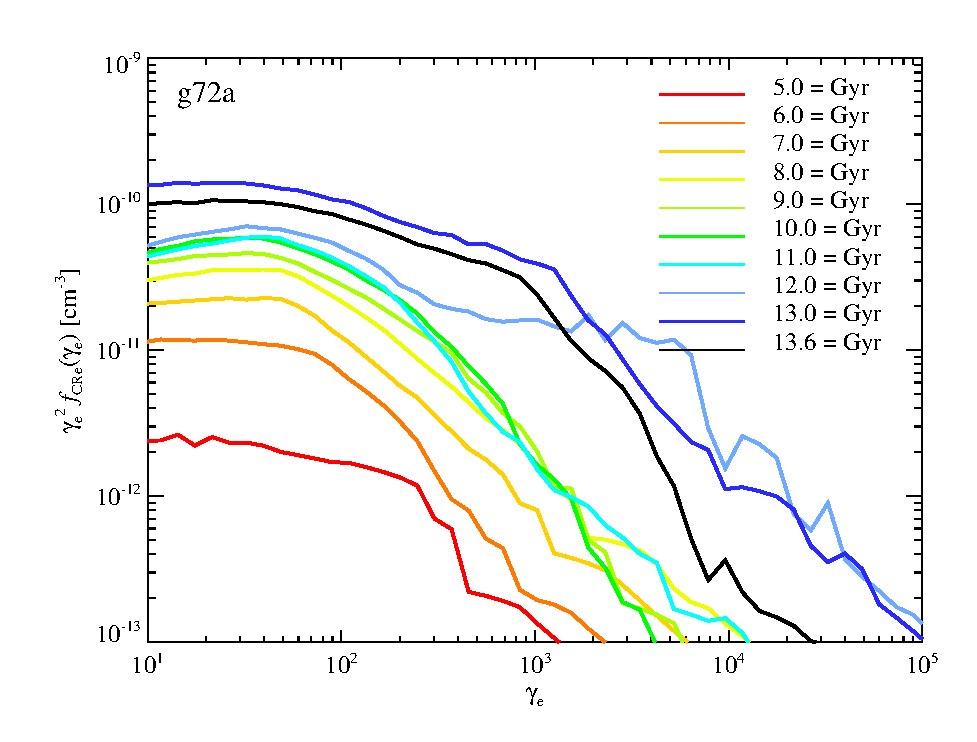
\includegraphics[width=0.32\columnwidth]{./figures/f_z.g72a.1.4Rv.a24.full.v20.eps}
  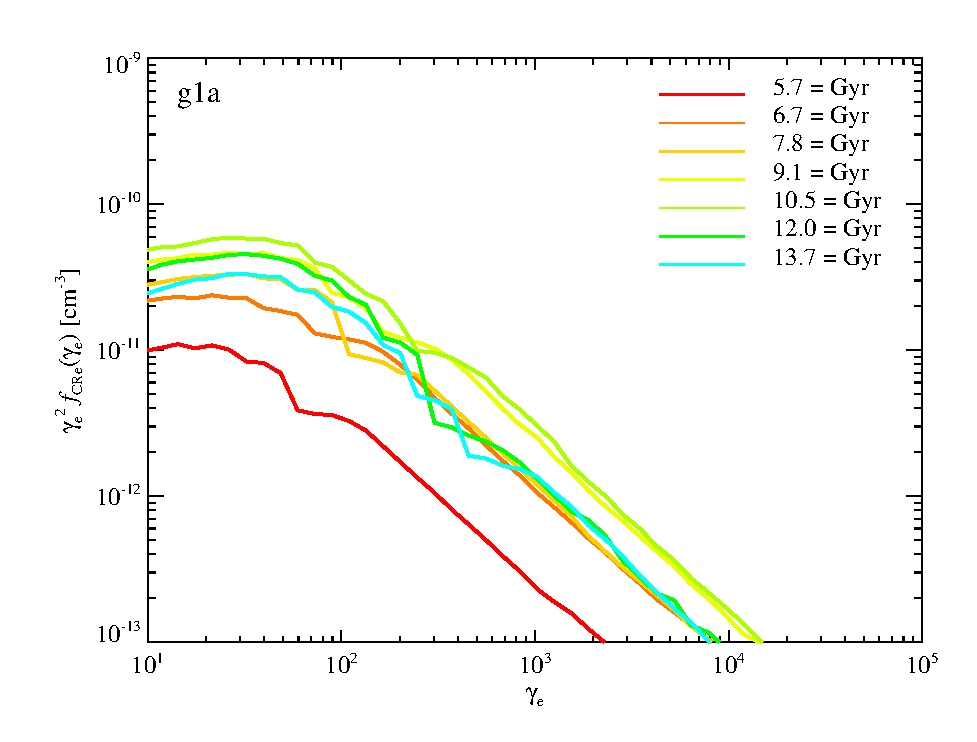
\includegraphics[width=0.32\columnwidth]{./figures/f_z.g1a.1.4Rv.a24.full.v20.eps}
  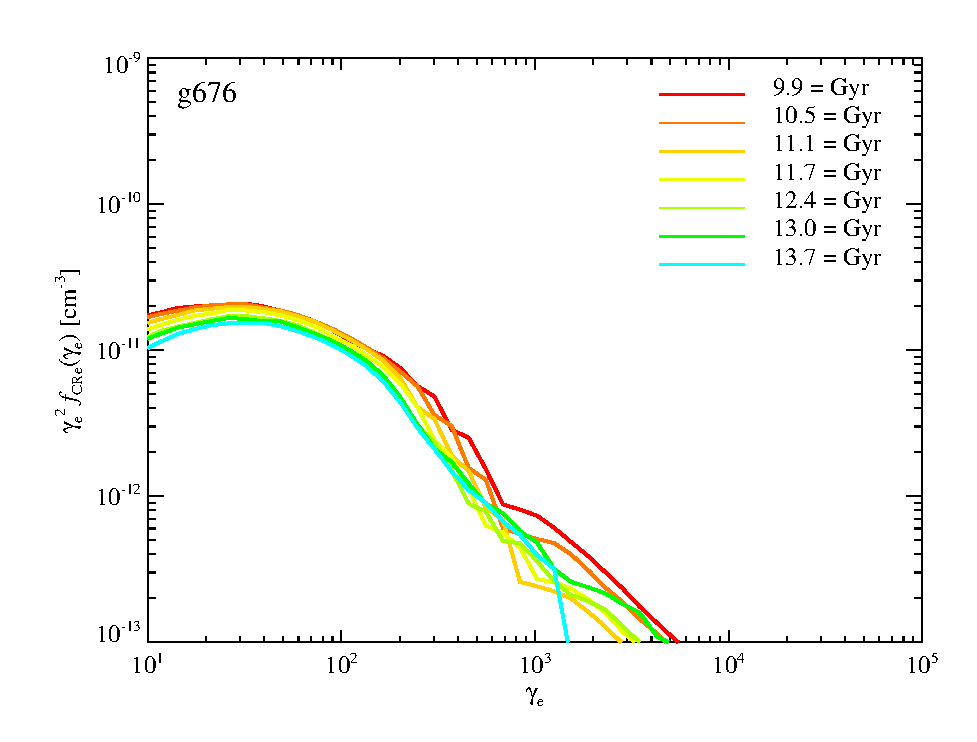
\includegraphics[width=0.32\columnwidth]{./figures/f_z.g676.1.4Rv.a24.full.v20.eps}
  \caption{Time evolution of the cosmic ray electron spectra in
    cluster outskirts. We show the total volume weighted CR electron
    distribution function for the particles that reside end up in
    region between (1.3-1.5)$\rvir$ at redshift zero; a cluster with a
    recent merger (g72a, left panel), large cooling flow cluster (g1a,
    middle panel), and a small cooling flow cluster (g676, right
    panel). The different line colors show the CR electron spectra at
    different look-back times, where the most recent spectrum in black
    is at 13.6 Gyrs. Notice the larger scatter in the merging cluster,
    and the relative small difference in the cooling flow
    clusters. The shape of the distribution function is very similar
    between different cooling flow clusters, and slightly more
    stochastic for merging clusters.\label{fig:e_spec_z}}
\end{minipage}
\end{figure*}

\begin{figure*}
\begin{minipage}{2.0\columnwidth}
  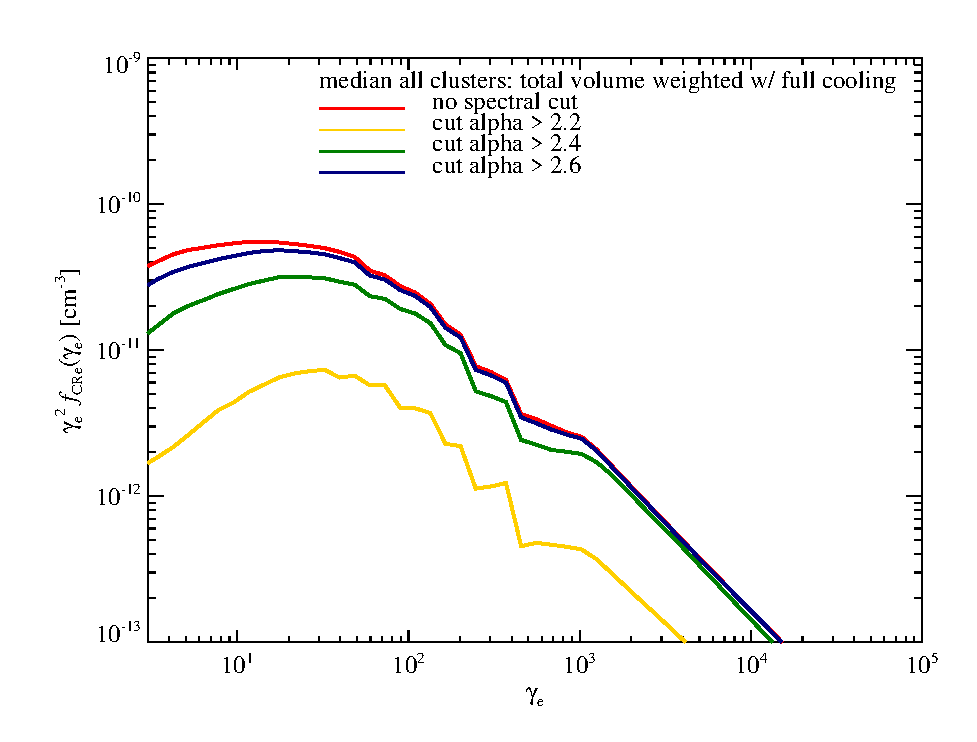
\includegraphics[width=0.49\columnwidth]{./figures/CRspec.alphaCheck.eps}
  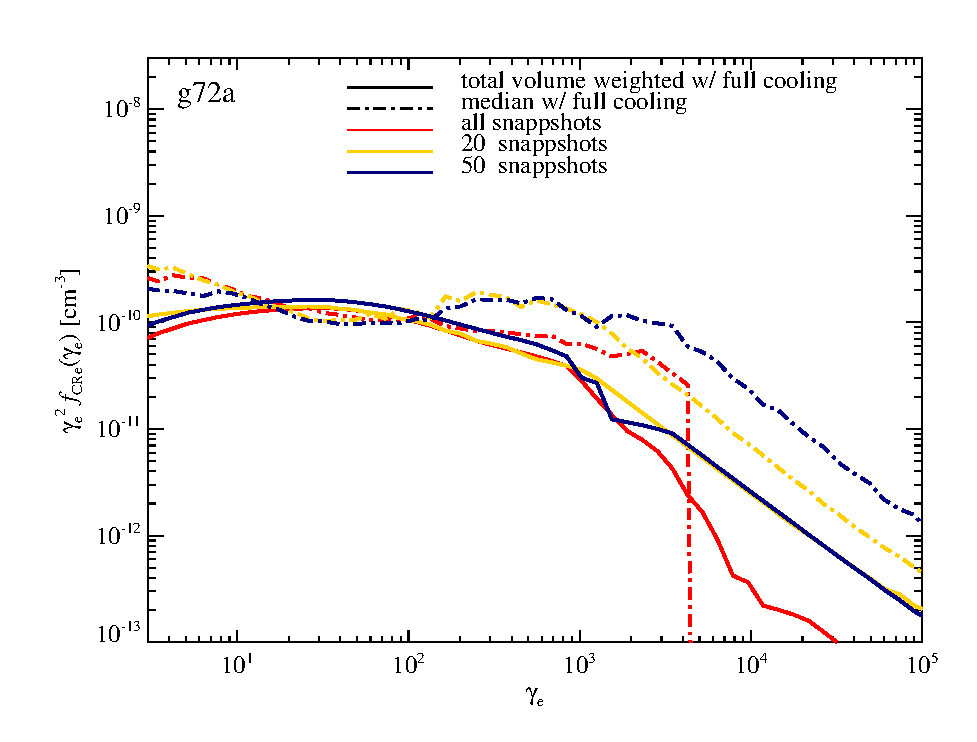
\includegraphics[width=0.49\columnwidth]{./figures/CRspec.snapCheck.eps}
  \caption{Testing the robustness of the CR electron spectra. Left
    panel shows how different cuts in injected spectra impact the
    total volume weighted CR electron spectrum with full cooling; no
    spectral cut (red line), cut particles with $\alpha_\inj>2.2$
    (yellow line), cut particles with $\alpha_\inj>2.4$ (green line),
    cut particles with $\alpha_\inj>2.6$ (blue line). Note that in the
    main CR model we cut all particles with an $\alpha_\inj>2.4$,
    which is a factor four smaller at low energies than the spectrum
    without a cut. Right panel shows the effect of time-resolution on
    the CR electron spectra. The median CR spectrum is shown with full
    cooling that includes radiative, Coulomb, and adiabatic losses
    (dash-dotted line), the solid line represents the total volume
    weighted CR electron spectrum with full cooling. The three line
    colors corresponds to the same cluster, a large coma like merging
    cluster, but with different time resolution between snapshots in
    the relevant regime; red lines corresponds to 100 Myrs between
    snapshots, orange lines corresponds to ~(1.0-1.5) Gyrs between
    snapshots, and the blue lines corresponds to ~(1.0-1.5) Gyrs
    between snapshots. \label{fig:e_spec_tests}}
\end{minipage}
\end{figure*}

\begin{figure*}
\begin{minipage}{2.0\columnwidth}
  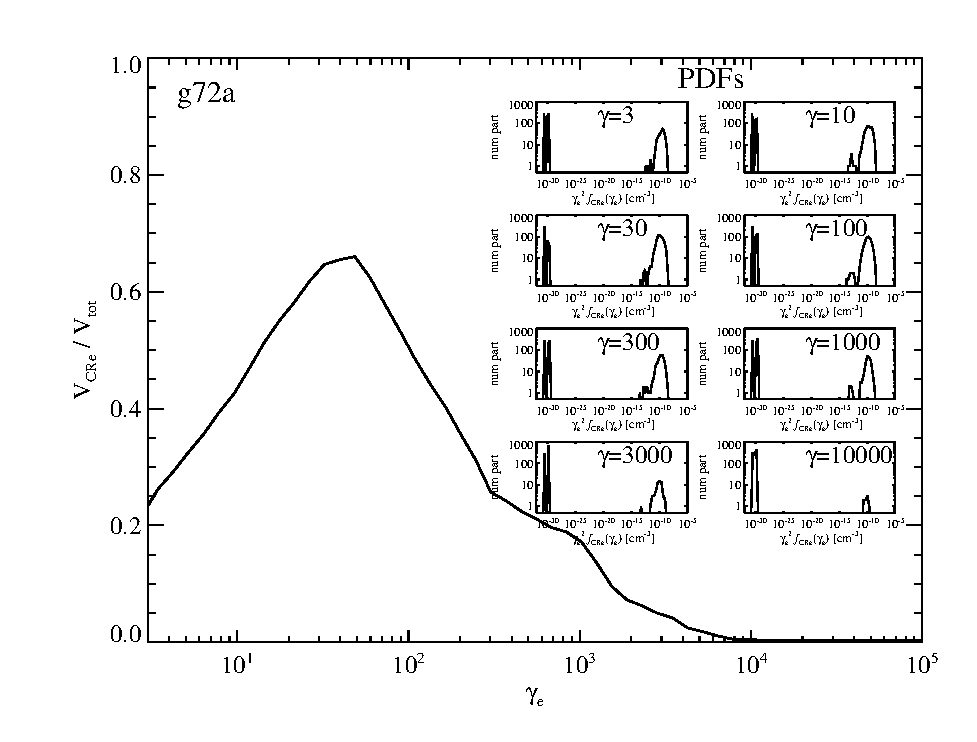
\includegraphics[width=0.49\columnwidth]{./figures/CRvolume.g72a.1.4Rv.a24.full.140.v20.eps}
  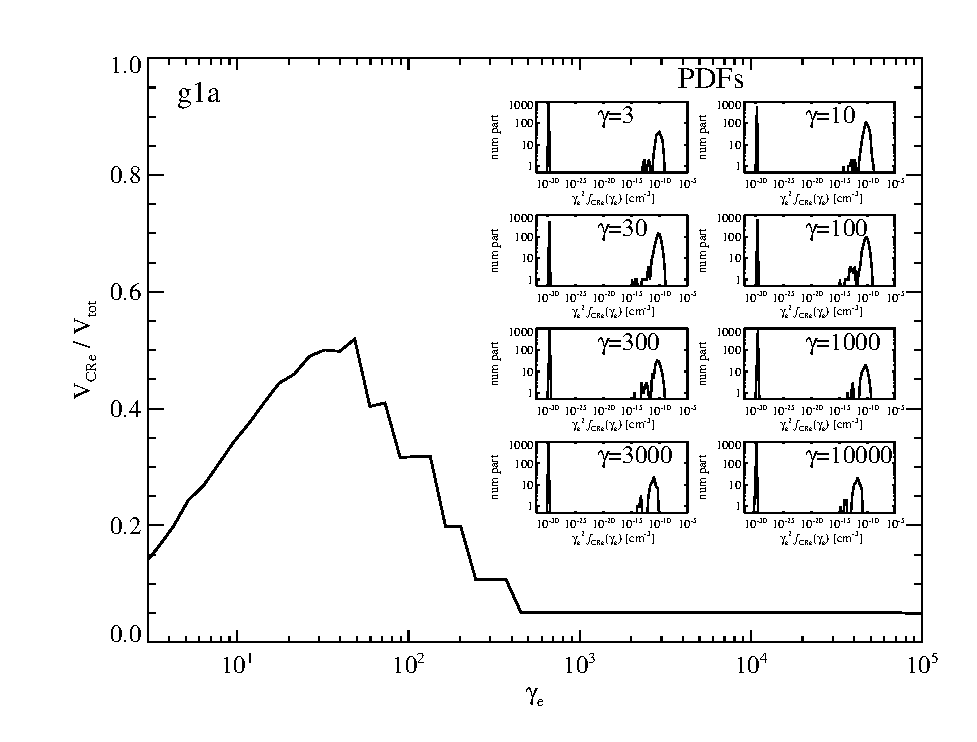
\includegraphics[width=0.49\columnwidth]{./figures/CRvolume.g1a.1.4Rv.a24.full.020.v20.eps}
  \caption{The fractional volume occupied by CR electrons in cluster
    outskirts. Large panels (left Coma like cluster, and right massive
    cooling flow cluster) show the fractional volume occupied by CR
    electrons as a function of logarithmic Lorentz factor ($\gam_\e$)
    in the region between (1.3-1.5)$\rvir$ at redshift zero. The
    smaller panels show the logarithmic particle distribution function
    for different $\gam_\e$, where the left peaks corresponds to
    unpopulated SPH particles and cooled CR particles, while the right
    peaks show the CR populated SPH
    particles. \label{fig:e_spec_CRvolume}}
\end{minipage}
\end{figure*}

\begin{figure}
  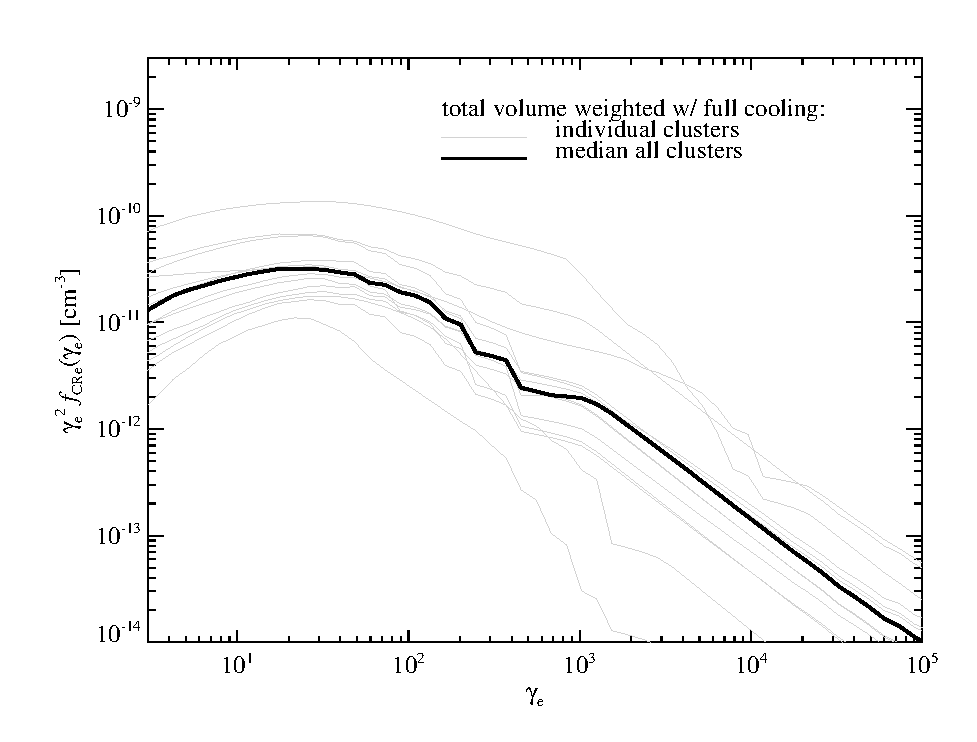
\includegraphics[width=1.0\columnwidth]{./figures/CRespec.all.1.4Rv.a24.full.020.v20.eps}
  \caption{Cosmic ray electron spectra in cluster outskirts at
    redshift zero. We show the total volume weighted CR electron
    distribution function in the region between (1.3-1.5)$\rvir$ with
    full cooling that includes radiative, Coulomb, and adiabatic
    losses. The the thin grey lines show the spectra from individual
    clusters while the thick solid line shows the median of the
    spectra from all clusters. \label{fig:e_spec_all}}
\end{figure}

\begin{figure}
  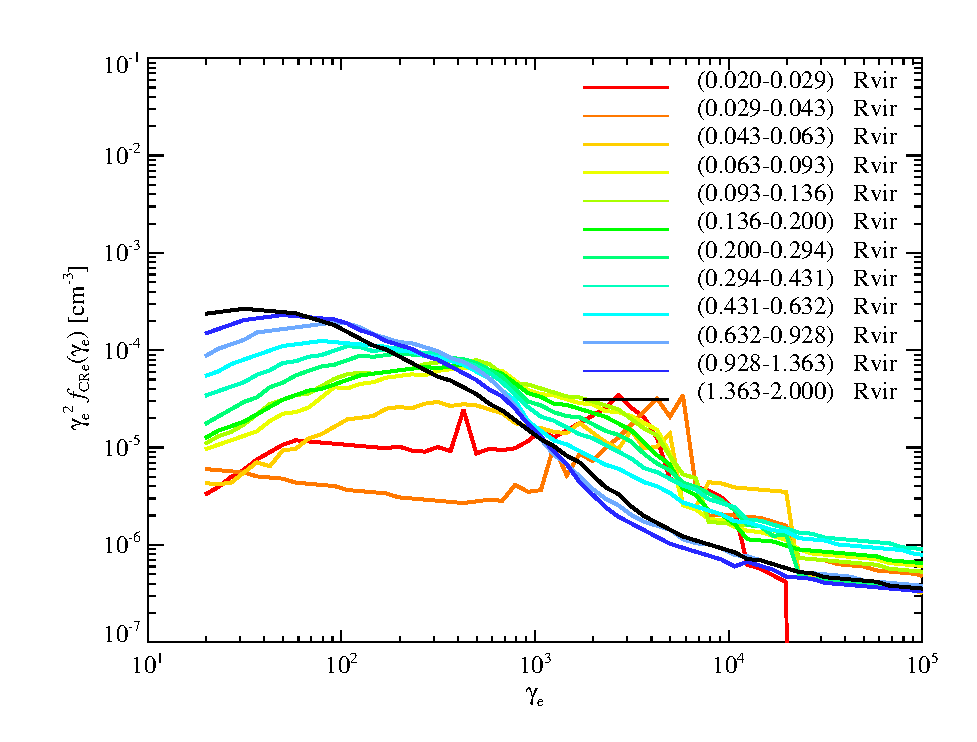
\includegraphics[width=1.0\columnwidth]{./figures/old/CRespecRadial.Radial2Rv.a24.140.v16.eps}
  \caption{Spatial dependence of the cosmic ray electron spectra at
    redshift zero. We show the total volume weighted CR electron
    distribution function; a Coma like cluster (left panel), a massive
    cooling flow cluster (middle panel), and the median of our 14
    cluster's spectra (right panel). The different line colors show
    the CR electron spectra for different radial
    bins.\label{fig:e_spec_spatial}}
\end{figure}

\begin{figure}
  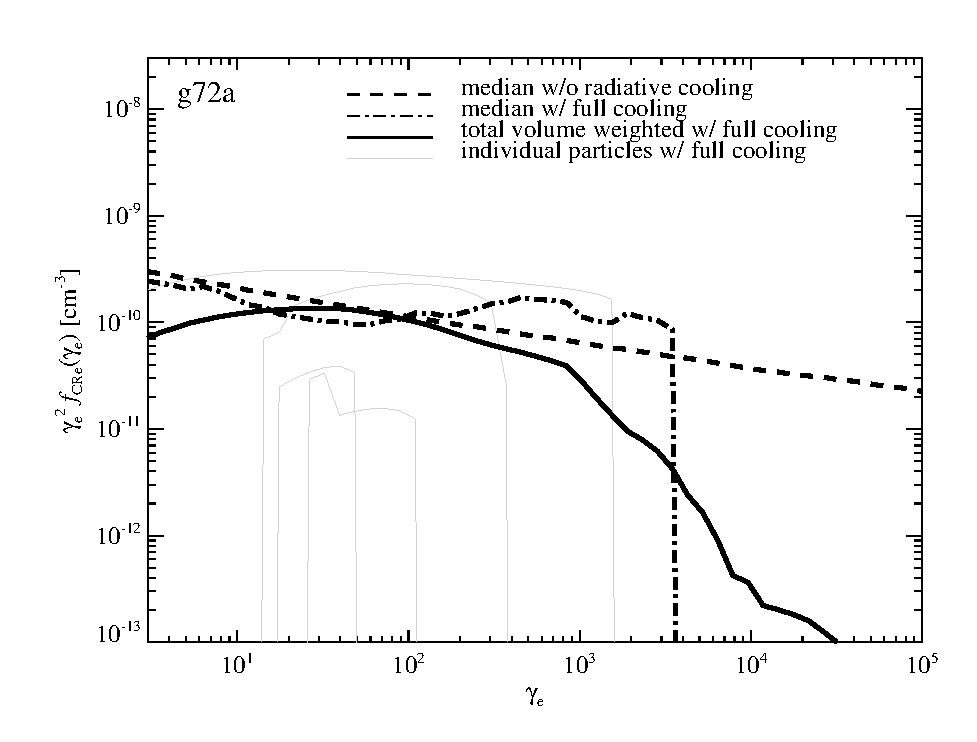
\includegraphics[width=1.0\columnwidth]{./figures/CRespec.g72a.1.4Rv.a24.full.140.v20.eps}
  \caption{Cosmic ray electron spectra in cluster outskirts at
    redshift zero. We show the CR electron distribution function
    weighted with the electron Lorentz factor ($\gam_\e$) squared for
    a typical cluster with a recent merger for region between
    (1.3-1.5)$\rvir$. The median CR spectrum is shown with full
    cooling that includes radiative, Coulomb, and adiabatic losses
    (dash-dotted line), and with only adiabatic losses (dashed
    line). The solid line represents the total volume weighted CR
    electron spectrum with full cooling. Note that the Coulomb cooling
    at low energies is very inefficient because of the low electron
    densities in the cluster outskirts.\label{fig:e_spec_g72a}}
\end{figure}

\del{
\begin{figure*}
\begin{minipage}{2.0\columnwidth}
%  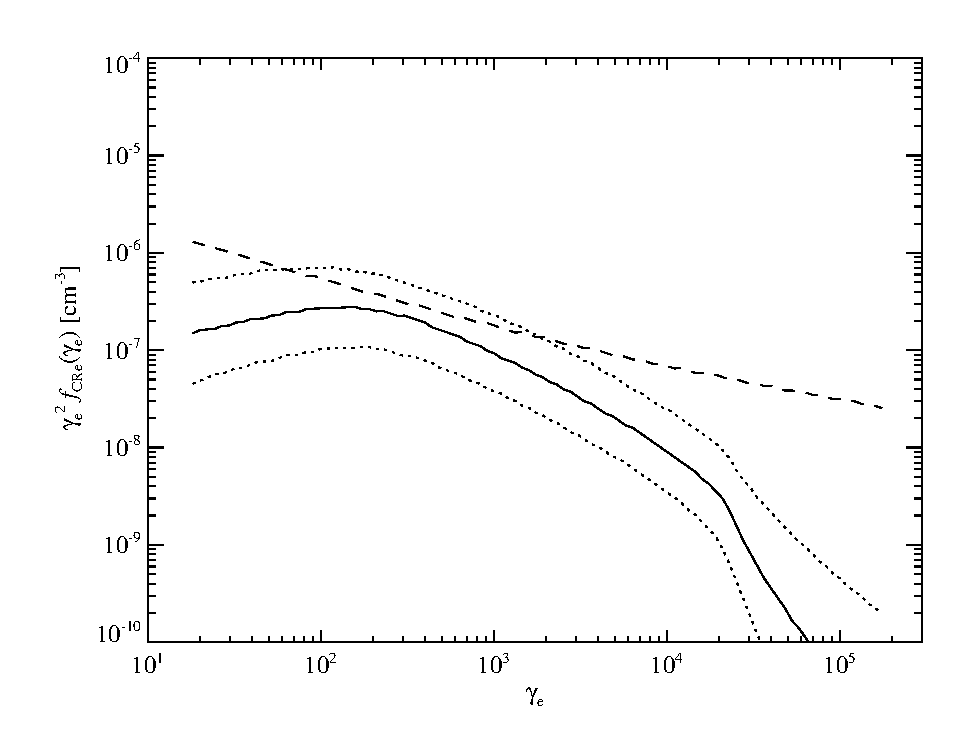
\includegraphics[width=0.49\columnwidth]{./figures/CRespec0.3Rv.140.v12.eps}
%  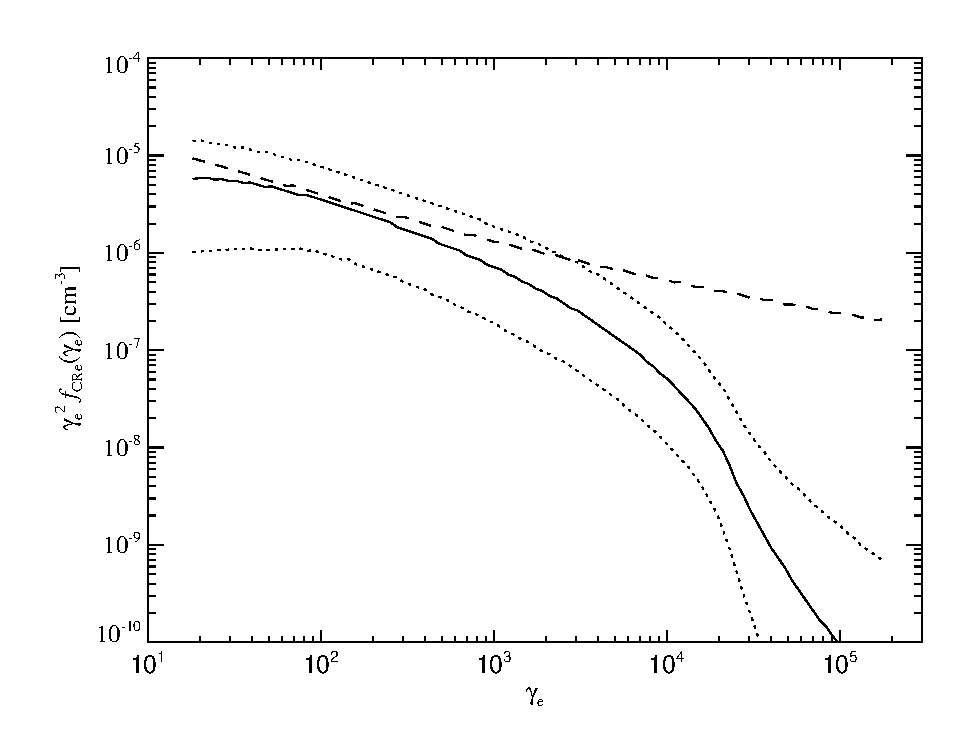
\includegraphics[width=0.49\columnwidth]{./figures/CRespec1.4Rv.140.v12.eps}
  \caption{Cosmic ray electron spectra in cluster outskirts at
    redshift zero. We show the CR electron distribution function
    weighted with the electron Lorentz factor ($\gam_\e$)
    squared. In the {\it left panel} panel we show the CR electron in
    the region between (0.3-0.5)$\rvir$ and in the {\it right panel}
    between (1.3-1.5)$\rvir$. The solid lines show the median CR
    electron spectrum where both radiative and adiabatic losses are
    included. The dotted lines shows the 68 percentiles. The dashed
    lines show the CR electron spectrum without Coulomb and radiative
    cooling. Note that the Coulomb cooling at low energies is very
    inefficient because of the low electron densities in the cluster
    outskirts. \label{fig:e_spec}}
\end{minipage}
\end{figure*}
}

\del{
\begin{figure*}
\begin{minipage}{2.0\columnwidth}
%  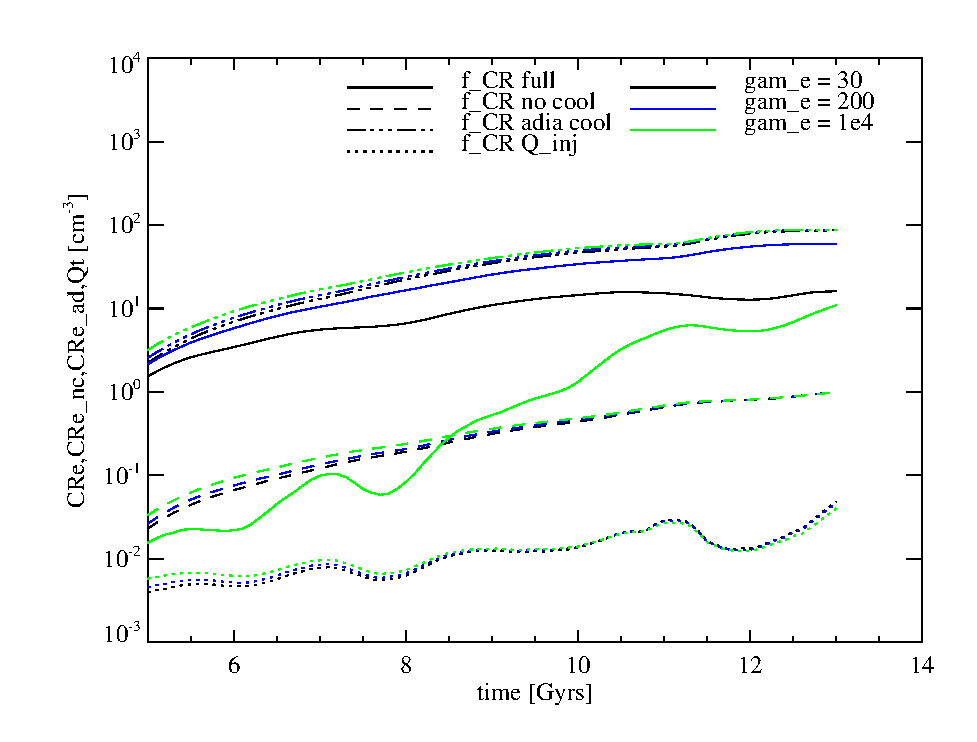
\includegraphics[width=0.49\columnwidth]{./figures/f_evolution.0.3Rv.eps}
%  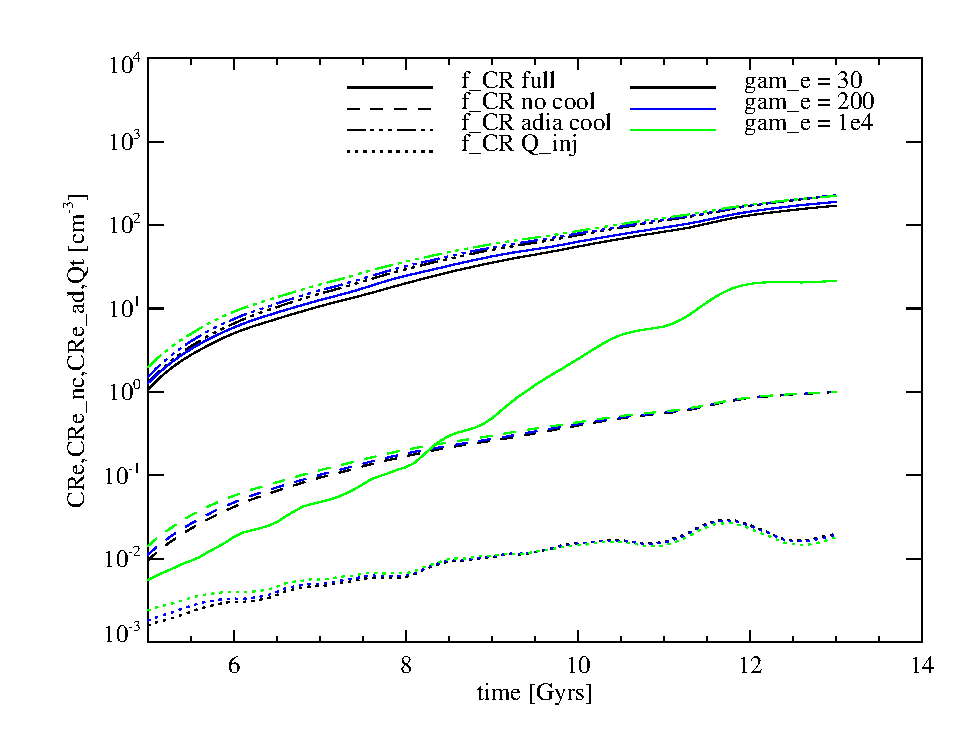
\includegraphics[width=0.49\columnwidth]{./figures/f_evolution.1.4Rv.eps}
  \caption{Time evolution of cosmic ray (CR) electron spectra. We show
    the CR electron distribution function weighted with the electron
    Lorentz factor ($\gam_\e$) squared. The time evolution of the CR
    electrons which at $z=0$ reside from (0.3-0.5)$\rvir$ are shown in
    the {\it left panel} and (1.3-1.5)$\rvir$ in the {\it right
      panel}. The black lines show the CR electrons with a
    $\gam_\e=30$, blue lines $\gam_\e=200$, and green lines
    $\gam_\e=10^4$. The solid lines show the CR electrons with full
    cooling, i.e. for Coulomb, inverse Compton, and adiabatic
    losses. Dashed lines show the CR electrons without Coulomb and
    inverse Compton cooling while the dash-dotted lines show the CR
    electrons without adiabatic cooling. The dotted line show the
    injected CR electron distribution function, derived from the
    injected CR protons. For each energy, we normalize the CR electron
    distribution function with the CR electrons without
    cooling. Notice that the high energy part is built up during the
    last Gyr. This is explained by the inverse Compton losses that are
    larger at high energies, especially at high redshifts where the
    energy density of the CMB is much larger than
    today.  \label{fig:e_evol}}
\end{minipage}
\end{figure*}
}

\del{
\begin{figure*}
\begin{minipage}{2.0\columnwidth}
%  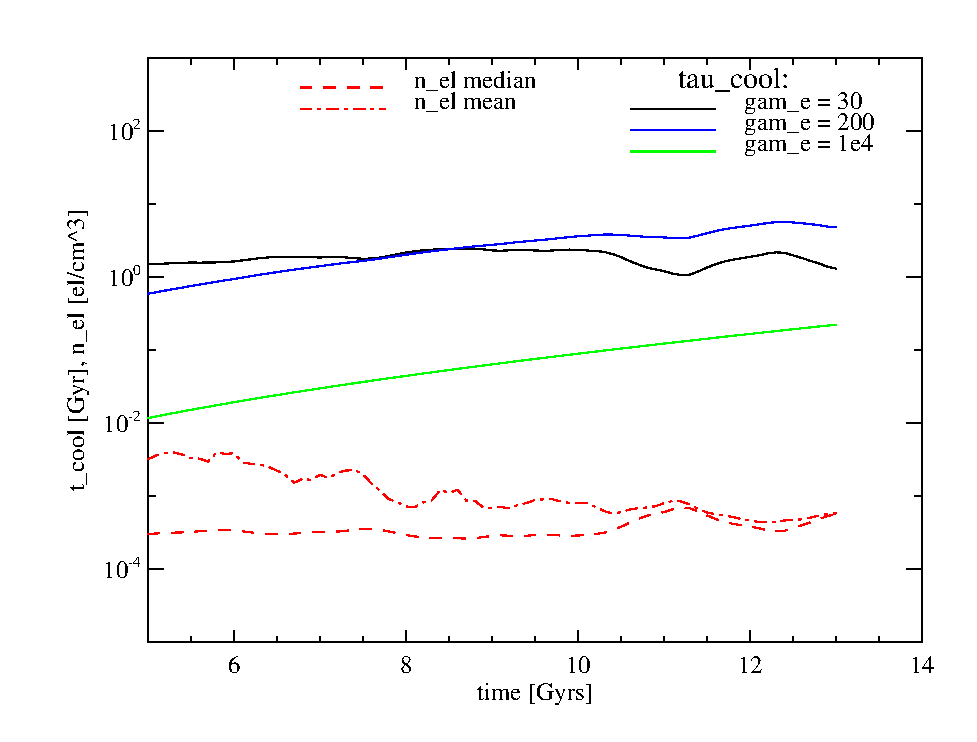
\includegraphics[width=0.49\columnwidth]{./figures/evolution.0.3Rv.eps}
%  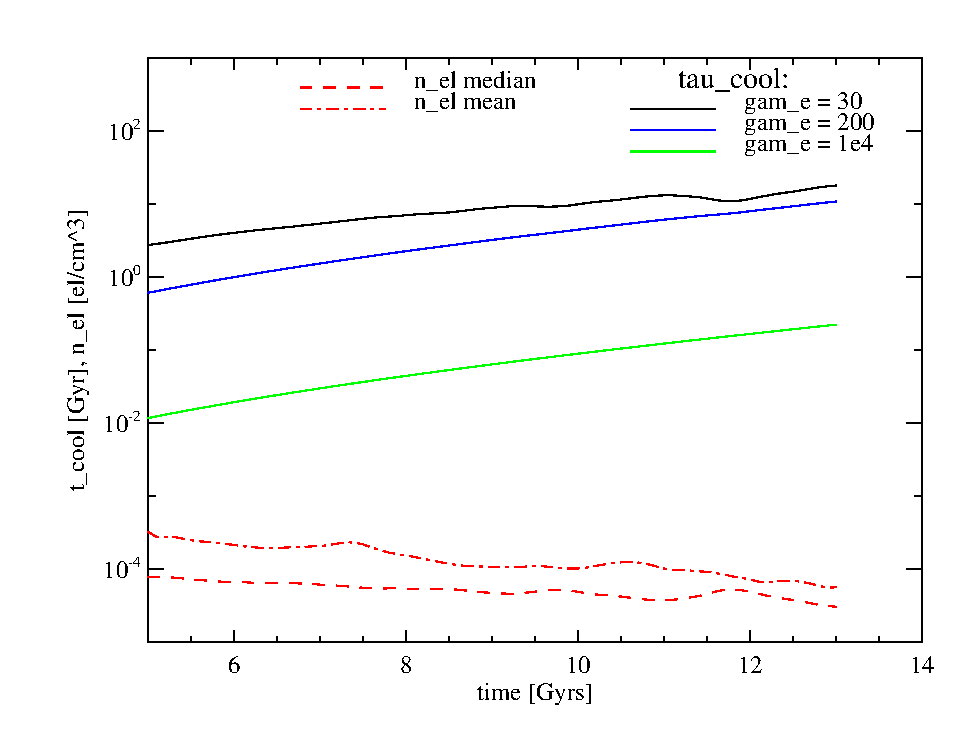
\includegraphics[width=0.49\columnwidth]{./figures/evolution.1.4Rv.eps}
  \caption{Time evolution of the gas density and the cosmic ray (CR)
    cooling time. We show the time evolution of the electron number
    density and CR electron cooling time that are associated with the
    CR electrons which at redshift $z=0$ reside from (0.3-0.5)$\rvir$
    in the {\it left panel} and (1.3-1.5)$\rvir$ in the {\it right
      panel}. The red lines show the electron number densities, where
    the dashed line show the median and dash-dotted the mean. The
    solid lines show the cooling times
    $\tau_\rmn{cool}=\gam_\e/[b_\IC(\gam_\e)+b_\rmn{C}(\gam_\e)]$
    for $\gam_\e=30$ (black), $\gam_\e=200$ (blue), and
    $\gam_\e=10^4$ (green). Interesting the CR cooling at low
    energies of the particles that end up in the center is constant
    while is increasing monotonically for the particles that end up in
    the cluster periphery. The density of the particles that end up in
    the center is roughly constant with time while it is decreasing
    for the particles that end up in the outer part. This is due to
    the expansion of the universe that counteract the contraction of
    the particles in the cluster periphery. \label{fig:evol}}
\end{minipage}
\end{figure*}
}

% --- section: --- %
\section{Conclusions}
\label{sect:conclusions}

% --- section: --- %
\section*{Acknowledgments}

% --- section: bibliography --- %
\bibliography{bibtex/paper}
\bibliographystyle{mn2e}

\appendix

\bsp

\label{lastpage}

\end{document}
